%!TEX root = ../my_thesis.tex
\chapter{Caractérisation, identification et correction des erreurs résiduelles} % (fold)
Ce chapitre troisième vise à présenter une méthode permettant de corriger les erreurs résiduelles rencontrées dans la zone
du plancher d'erreur lors du décodage des turbo codes.

Suite à une observation de ces erreurs, une prédiction de leurs distributions basée sur la borne de l'union est proposé. 
Ceci permet alors de les caractériser.

Dans un second temps, plusieurs critères d'identification sont proposés et comparés. Ceux-ci 
sont aussi bien adaptés aux turbo codes binaires qu'aux double binaires.

Ceci mène alors à la proposition d'un algorithme permettant de corriger les erreurs résiduelles des turbo codes.
Il a pour propriété d'abaisser drastiquement le plancher d'erreurs lors du décodage des turbo codes.
Une comparaison avec l'état de l'art met en exergue l’intérêt de cette approche.


\vspace*{\fill}
\minitocTITI
\vspace*{\fill}
\newpage

\section{Analyse des erreurs résiduelles}
\subsection{Caractérisation théorique}
Comme présenté dans le chapitre premier, l'apparition du plancher d'erreur dépend de la distribution des mots de codes 
possédant un faible poids \cite{distance_spectrum}. Plus encore, il a été montré que la zone du plancher d'erreur émanait 
de la présence \emph{d'erreurs résiduelles} \cite{takeshitaBCH}. 
La Figure \ref{fig:befe} présente l'évolution du nombre moyen de bits erronés par trame erronée en fonction de la valeur de 
SNR pour cinq turbo codes binaires différents. Quatre de ces codes appartiennent au standard LTE, le cinquième au standard CCSDS. 
À chaque fois, une rendement de 1/3 et un turbo décodage basé sur l'algorithme EML-MAP itérant 8 fois sont considérés. Dans la zone de 
convergence, de nombreuses erreurs à l'issu du décodage sont présentes. En revanche, dès lors que le décodeur 
fonctionne dans la zone du plancher d'erreurs, le nombre moyen d'erreurs binaires par trame erronée est inférieur à 10. 
De là vient leur nom d'erreurs résiduelles.

\begin{figure}[!b]
	\centering
	\includegraphics[width=.8\textwidth]{main/ch3_fig/be/tikz/befe.pdf}
	\caption{Évolution du nombre moyen d'erreurs binaires par trame erronée pour différentes valeurs de SNR et différents
	turbo codes. Décodage effectué par l'algorithme EML-MAP itérant 8 fois. \label{fig:befe}}
\end{figure}

Une caractérisation de la distribution de ces erreurs 
résiduelles a été proposée dans \cite{residual_errors}. Cette dernière est basée sur les fonctions recenseuses de poids
(Weight Enumerator Functions ou WEF en anglais, \cite{ryan}). En posant $P^{\langle ML\rangle}(m)$ la probabilité que 
$m$ bits soient erronés dans une trame et sachant que la trame est erronée après un décodage à maximum de vraisemblance,
l'expression suivante est obtenue :
\begin{equation}
P^{\langle ML\rangle}(m) \simeq \frac{W^m~A_m^{\langle CP\rangle}(Z)\vert_{W=Z=e^{-RE_b/N_0}}}{\sum\limits_{w=1}^N W^w~A_w^{\langle CP\rangle}(Z) \vert_{W=Z=e^{-RE_b/N_0}}}
\label{eq:be1}
\end{equation}
où $A_w^{\langle CP\rangle}(Z)$ est le WEF conditionnel du turbo code considéré \cite{benedetto_unveiling}.

En supposant que les séquences d'information 
générant un mot de code de poids $w$ ont majoritairement le même poids, l'équation précédente peut alors être transformée 
en : 
\begin{equation}
P^{\langle ML\rangle}(m) \approx \frac{\displaystyle\sum\limits_{w, \frac{W_w}{A_w}=m} A_w\cdot \exp\left(-w R \frac{E_b}{N_0}\right)}
                  {\displaystyle\sum\limits_{w} A_w\cdot \exp\left(-w R \frac{E_b}{N_0}\right)}
\label{eq:be2}
\end{equation}
avec, comme déjà présenté dans le Chapitre Premier, $A_w$ le nombre de mots de code de poids de Hamming $w$. La 
multiplicité des bits d'information $W_w$ est la somme des poids de Hamming des $A_w$ séquences binaires générant des
mots de code de poids de Hamming $w$. Au prix d'une faible imprécision, cette forme de l'équation permet d'utiliser 
directement le spectre de distance d'un turbo code pour estimer le nombre de bits erronées dans le plancher d'erreur. Les
résultats obtenus avec cette équation différent alors légèrement de ceux obtenus avec l'Équation \ref{eq:be1}. En effet,
certaines valeurs sont masquées par l'opération de moyenne : $\frac{W_w}{A_w}=m$. 

Ainsi, le spectre de distance d'un turbo code permet de calculer la probabilité 
d'obtenir $m$ erreurs binaires dans une trame erronée en considérant un décodage ML pour un taux d'erreur suffisamment 
faible et un canal AWGN. De part la présence du terme en exponentielle, plus le poids du mot de code $w$ est distant 
de $d_{min}$, moins la multiplicité associée a un impact sur la distribution des erreurs résiduelles. Ceci peut néanmoins
être fortement atténué par une multiplicité très importante (de l'ordre du millier, rencontré fréquemment lors des 
expérimentations).

% Dans la section suivante, grâce à l'obtention des spectres de distances de différents turbo codes standardisés, une 
% comparaison est menée quant à la distribution du nombre d'erreurs dans les trames erronées dans la zone du plancher 
% d'erreurs.
Dans la section suivante, ces résultats théoriques sont comparés à des distributions observées du nombre d'erreurs dans les
trames erronées de la zone du plancher d'erreur avec un décodage basé sur l'algorithme ELM-MAP.

\subsection{Observations considérant des turbo codes standardisés}
L'existence des erreurs résiduelles dans la zone du plancher d'erreur a été théoriquement établie. L'obtention 
de la distribution de ces erreurs est maintenant proposée. Dans un premier temps, des turbo codes binaires de tailles de 
trames différentes et de rendement 1/3 sont considérés. Dans un second temps, des turbo codes double binaires d'un seule 
taille de trame mais de différents rendements sont considérés. Ainsi, un large spectre de paramètres sont exploités sans
présenter un nombre trop conséquent de données.

\subsubsection{Dans le cas de turbo codes binaires}

La Figure \ref{fig:be} présente la distribution des erreurs résiduelles pour 5 turbo codes du standard LTE et un du 
standard CCSDS. Le rendement du code est fixé à 1/3. Pour chacun de ces histogrammes, 500 trames erronées
après décodage via l'algorithme EMNL-MAP itérant 8 fois sont considérées. Il apparaît alors que la très grande majorité 
des trames erronées contiennent moins de 10 erreurs binaires. 
%Ceci est conforté par la Figure \ref{fig:befe}. 
Plus encore, hormis pour le turbo code du standard CCSDS, 70\% des trames erronées ont strictement moins de 5 erreurs.

\begin{figure}[!ht]
	\centering
	\hspace*{-1cm}
	\includegraphics[width=1.07\textwidth]{main/ch3_fig/be/tikz/be.pdf}
	\caption{Distribution du nombre d'erreurs binaires pour différentes valeur de SNR et pour différents turbo codes des 
	standards LTE et CCSDS. 
	Décodage EML-MAP itérant 8 fois. \label{fig:be}}
\end{figure}

Sont aussi présentés sur la Figure \ref{fig:be} les résultats théoriques obtenus pour la valeur de SNR la plus grande
grâce à l'équation \ref{eq:be1} et au spectre de distance calculé via la Double Impulse Method (cf. \ref{seq:spectre}).
Ces résultats sont reportés pour plus de lisibilité dans le Tableau \ref{tab:theo}. Suivant le turbo code considéré,
des différences entre la valeur théorique et la valeur mesurée apparaissent. Néanmoins, la tendance pour les valeurs
calculées est conforme
aux mesures obtenues. Ainsi, la seule occurrence non prédite correspond à un BE de 1 pour le standard CCSDS, où $0.2\%$ 
était prédit alors que $11\%$ sont mesurés.

\begin{table}[]
\centering
\caption{Distribution théorique des erreurs dans le plancher d'erreur selon l'équation \ref{eq:be1} pour différents turbo 
codes standardisés}
\label{tab:theo}
\resizebox{\textwidth}{!}{
\begin{tabular}{@{}lrrrrrrrrrrr@{}}
\toprule
                            & 1      & 2      & 3      & 4      & 5     & 6      & 7     & 8      & 9     & 10  & \textgreater10 \\ \cmidrule(r){1-1} \cmidrule(l){2-12}
LTE R=1/3, K=528 @ 2.4dB    & 33.9\% & 24.4\% & 29.3\% & 1.4\%  & 1\%   & 5.2\%  & 0.2\% & 0.02\% & 4.6\% & 0\% & 0\%            \\
LTE R=1/3, K=1024 @ 1.5dB   & 19.9\% & 32.7\% & 36.7\% & 6.2\%  & 3.6\% & 0.3\%  & 0.4\% & 0.2\%  & 0\%   & 0\% & 0\%            \\
LTE R=1/3, K=1504 @ 1.3dB   & 0\%    & 19.2\% & 68\%   & 8.3\%  & 2.2\% & 0.8\%  & 1.4\% & 0\%    & 0\%   & 0\% & 0\%            \\
LTE R=1/3, K=2048 @ 1.3dB   & 26\%   & 33.7\% & 30.2\% & 7.9\%  & 1.4\% & 0.3\%  & 0.4\% & 0.1\%  & 0\%   & 0\% & 0\%            \\
LTE R=1/3, K=6144 @ 0.8dB   & 0\%    & 76\%   & 7.2\%  & 14.2\% & 2.1\% & 0.3\%  & 0.1\% & 0\%    & 0\%   & 0\% & 0\%            \\
CCSDS R=1/3, K=1784 @ 1.3dB & 0.2\%  & 48.1\% & 27.9\% & 0.2\%  & 0.1\% & 22.3\% & 0.1\% & 0.1\%  & 0.6\% & 0\% & 0\%            \\ \bottomrule
\end{tabular}}
\end{table}

Afin de présenter la déviation entre la théorie développée dans la première section de ce Chapitre et les mesures 
effectuées, un calcul d'erreur quadratique moyenne (EQM, Équation \ref{eq:eqm}) est effectué pour chacun des turbo codes. 
Les valeurs obtenues sont récapitulées dans le tableau \ref{tab:eqm}.

\begin{equation}
	EQM = \sqrt{\cfrac{1}{N}\sum\limits_{i=1}^N\bigl(T_i-M_i\bigr)^2}
	\label{eq:eqm}
\end{equation}

Les valeurs d'EQM sont alors comprises entre 3.8 et 9.5, impliquant que les valeurs théoriques et mesurées sont 
relativement proches. Ainsi même si des écarts apparaissent, ces équations permettent de prédire l'allure de la distribution
des erreurs binaires dans la zone du plancher d'écart. Les écarts s'expliquent par le fait que les Équations \ref{eq:be1} 
et \ref{eq:be2} ne sont vraies que dans le cas d'un décodage ML. Or ce dernier ne peut pas être effectué dans le contexte des turbo codes.

Plus le ratio $\frac{W_d}{A_d}$ des premiers termes du spectre de distance du code est faible, plus le nombre moyen de 
bit erronés par trame erronée dans le plancher d'erreur sera faible lui aussi. Pour les turbo codes 
standardisés, les ratios $\frac{W_d}{A_d}$ sont habituellement faibles. Ceci implique alors une distribution des erreurs 
binaires dans le plancher d'erreur centrée sur les faibles nombres d'erreurs.
\begin{table}[b]
\centering
\caption{Erreur quadratique moyenne entre les valeurs théoriques et les simulations Monte-Carlo}
\label{tab:eqm}
\resizebox{.4\textwidth}{!}{
\begin{tabular}{@{}lr@{}}
\toprule
                            & EQM \\
                      \cmidrule(r){1-1}      \cmidrule{2-2}
LTE R=1/3, K=528 @ 2.4dB    & 6.2 \\
LTE R=1/3, K=1024 @ 1.5dB   & 9.4 \\
LTE R=1/3, K=1504 @ 1.3dB   & 9.5 \\
LTE R=1/3, K=2048 @ 1.3dB   & 3.8 \\
LTE R=1/3, K=6144 @ 0.8dB   & 6.7 \\
CCSDS R=1/3, K=1784 @ 1.3dB & 6.9 \\
\bottomrule
\end{tabular}}
\end{table}

Maintenant, une analyse similaire vient confirmer étendre ces résultats dans le contexte de turbo codes double binaires.

\subsubsection{Dans le cas de turbo codes double binaires}
TODO la même chose : \\
Distribution des erreurs pour 4 turbo doubles binaires. K=1/3 1/2 3/4 6/7 (=0.33, 0.5, 0.75, 0.85)
																			0.17    0.25   0.1  2/3 aurait été mieux ?	
Spectre en annexe.\\
tableau EQM\\



Finalement, lorsqu'un processus de décodage itératif échoue dans le plancher d'erreur, la trame résultante est très proche du 
mot de code transmis. Cette constatation semble vraie pour tout turbo code standardisé, incluant les turbo codes
double binaires. Dans la section suivante, différents critères d'identification de ces erreurs résiduelles sont 
proposés et comparés.
\newpage
\section{Comparaison de critères d'identification}
Dans cette section, une comparaison de plusieurs métriques permettant l'identification des erreurs résiduelles est 
proposée. Ces différentes métriques sont basées sur des quantités internes du turbo décodeur qui seront détaillées ci-après.\\
Suite aux résultats obtenus dans le chapitre deuxième des métriques reposant sur des oscillations sont écartées. Ainsi, 
seules des métriques prenant en compte l'amplitude d'informations internes au turbo décodeurs sont privilégiées.

\subsection{Les différentes métriques considérées pour les turbo codes binaires}
Dans le Chapitre précédent, il a été introduit que le module de l'information \textit{a posteriori} peut être vu comme 
l'assurance du turbo décodeur sur sa décision quant à un certain bit du mot décodé. Ainsi, une première métrique pouvant 
être établie est la suivante :
\begin{equation}
	\Delta_1(k) = |L^a(k)|\text{~, avec k~}\in \llbracket0;~K \rrbracket 
\end{equation}
Par ailleurs, il peut être considéré que de décorréler les informations du canal pour la métrique peut être intéressant. En effet, 
cela permet d'exprimer seulement l'avis propre au décodeur. Cette métrique est alors uniquement basée sur les informations 
extrinsèques et a pour expression : 
\begin{equation}
	\Delta_2(k) = |L^e_{12}(k)+L^e_{21}(k)|
\end{equation}
D'autre part, il peut être intéressant de considérer une norme au sens mathématique. L'évaluation de la norme 1 
(distance de Manhattan) est suffisante puisque son emploi vis à ordonner des positions. En effet, l'ordre est 
conservé quelque soit la norme p ($p \in \mathbb{N} $) employée. Les expressions des deux équations précédentes deviennent 
alors respectivement :
\begin{equation}
	\Delta_3(k) = |y^s(k)| + |L^e_{12}(k)| + |L^e_{21}(k)|
\end{equation}
et 
\begin{equation}
	\Delta_4(k) = |L^e_{12}(k)| + |L^e_{21}(k)|
\end{equation}

Pour l'ensemble de ces métriques, les positions les moins fiables sont extraites en identifiant les positions les 
minimisant.

\subsubsection{Résultats d'identification}
Afin de comparer ces différentes métriques, des statistiques d'identification vont être exploitées. Le protocole 
expérimental est le suivant. Après chaque itération du processus de turbo décodage, les $n$ positions les moins fiables
dans la trame sont identifiées grâce à chacune de ces métriques. Si l'ensemble des erreurs est présent dans ces $n$ éléments,
alors l'identification est considérée comme réussie. Les turbo codes considérés sont des turbo codes binaires du standard LTE.
Plusieurs valeurs de SNR sont successivement étudiées. Afin 
d'obtenir des données valides, 500 trames erronées après un décodage par l'algorithme EML-MAP itérant 8 fois sont
observées.

La Figure \ref{fig:id1024} présente les résultats pour le turbo code LTE avec K=1024 et R=1/3. Les profondeurs de recherches 
considérées $n$ s'étalent de 4 à 20. Il apparaît tout d'abord que 
les deux critères d'identification basés sur une norme ($\Delta_3$ et $\Delta_4$) présentent les moins bonnes performances.
 Ceci peut être interprété en remarquant que les normes ne permettent pas d'identifier les
cas où chaque décodeur possède un avis ferme (forte amplitude) mais différent l'un de l'autre (signes opposés). Les deux 
autres métriques identifient en revanche ces cas possibles. La même constatation est faite pour d'autres turbo codes. 
Ainsi, l'utilisation d'une norme (au sens mathématique) est écartée dans la suite, ce au profit des métriques $\Delta_1$ 
et $\Delta_2$.

Ces deux dernières possèdent des performances proches avec un avantage pour la métrique $\Delta_1$. Il est à noter que le pouvoir 
d'identification de ces deux métriques augmente lorsque la valeur de SNR augmente. Ceci est corrélé avec la diminution du 
nombre moyen d'erreurs binaires par trame constatée dans la section précédente.

Toujours en considérant la Figure \ref{fig:id1024}, selon la profondeur de recherche employée et pour une valeur de SNR 
de 1.1 dB, entre 10 et 30\% des trames ont l'ensemble de leurs erreurs binaires identifiées. Ces taux ne 
permettent pas de proposer une correction intéressante. En effet, en supposant que ces 30\% de trames dont les erreurs sont 
identifiées soient effectivement corrigées par un mécanisme basé sur cette métrique, le taux d'erreur trame passerait alors 
de $2.3\times 10^{-4}$ à $1.6\times 10^{-4}$. L'amélioration des performances serait alors toute relative.

En considérant maintenant une valeur de SNR de 1.3 dB, le taux d'identification maximal atteint 65\% pour $n=20$ avec la 
métrique $\Delta_1$. Le taux d'erreur trame résultant passerait alors de 
$1.5\times 10^{-5}$ à $5.2\times 10^{-6}$. Cette fois, des gains substantiels sont possibles. D'après les données de la 
Figure \ref{fig:be}, dans ce même cas expérimental, 71\% des trames ont 20 erreurs ou moins. 
L'emploi de la métrique $\Delta_1$, semble alors permettre d'identifier l'ensemble des erreurs de 91\% des trames ayant 
moins de 20. Ce taux s'établit à 83\% pour la métrique $\Delta_2$. 
%Il apparaît donc que le pouvoir d'identification de ces métriques est important.
%En effet, seules de rares trames à faibles erreurs binaires n'ont pas eu la position 
% de leurs erreurs identifiées. Ainsi, les performances de la métrique sont d'autant plus importantes que le nombre de bits
% erronés par trames erronées est faible. Cette assertion est vérifiée avec la valeur de SNR la plus élevée considérée.
Il apparaît donc que seules de rares trames à faible nombre d'erreurs binaires n'ont pas l'ensemble de leurs erreurs
identifiées. Il est alors attendu que plus la valeur de SNR augmente, plus le nombre d'erreur binaire par trame erroné 
baisse. Par conséquent, les métriques identifient encore plus d'erreurs.

Ceci est vérifié, pour une valeur de SNR de 1.5 dB. Avec une profondeur de recherche fixée à $10$, 87,6\% des 
trames erronées ont l'intégralité de leurs erreurs identifiées grâce à la métrique $\Delta_2$. Ce taux atteint 89,4\% avec 
la métrique $\Delta_1$. Pour cette valeur de SNR, 93.8\% des trames possède 10 erreurs ou moins. Ainsi, les métriques 
permettent une identification quasiment parfaite de la position des erreurs résiduelles. Finalement, si chaque trame 
erronée dont la totalité des erreurs sont identifiées est corrigée, le taux d'erreur trame résultant passe de 
$3.6\times 10^{-6}$ à une valeur comprise entre $3.8\times 10^{-7}$ et $4.4\times 10^{-7}$ suivant la métrique $\Delta_1$ 
ou $\Delta_2$ employée.

\begin{figure}[!htb]
	\centering
	\includegraphics[width=.75\textwidth]{main/ch3_fig/id2/tikz/1024.pdf}
	\caption{Pourcentage d'identification pour le turbo code du standard LTE K=1024, R=1/3.
	Décodage EML-MAP itérant 8 fois. \label{fig:id1024}}
		%\vspace*{-1cm}
\end{figure}
%\newpage
La Figure \ref{fig:idLTE} présente les statistiques d'identification réussies pour trois autres turbo codes du standard 
LTE. Dans les trois cas considérés, les observations faites lors de l'analyse de la Figure \ref{fig:id1024} peuvent être 
vérifiées. Ces histogrammes valident donc la pertinence des métriques $\Delta_1$ et $\Delta_2$ pour l'identification des bits 
erronés lors du processus itératif de décodage. Dans tous les cas, pour des valeurs de SNR correspondant à un fonctionnement des 
turbo décodeurs dans la zone du plancher d'erreur, au moins 90\% des trames erronées ont l'ensemble de leurs erreurs 
identifiées par la métrique $\Delta_1$ pour un profondeur de recherche de taille 6.

Dans la section suivante, les métriques proposées sont étendues et caractérisées pour des turbo codes double 
binaires.

\begin{figure}[!h]
	\centering
	\hspace*{-1cm}
	\includegraphics[width=1.05\textwidth]{main/ch3_fig/id2/tikz/lte.pdf}
	\caption{Pourcentage d'identification pour différents turbo codes du standard LTE K=528, K=2048 et K=6144 avec R=1/3.
	Décodage EML-MAP itérant 8 fois. \label{fig:idLTE}}
\end{figure}

\subsection{Extension des critères d'identification aux turbo codes double binaires}
Le décodage des turbo codes double binaires a été détaillé en section \ref{sec:dbl}. Pour rappel, lors de ce décodage par
l'algorithme EML-MAP, 4 valeurs extrinsèques sont échangées pour chaque symbole. En réalité, dans un but de simplification de 
l'architecture matérielle associée, seules trois valeurs sont échangées puisqu'une normalisation vis-à-vis de 
la probabilité d'obtenir le symbole $\mathbf{0}$ est réalisée. 

La généralisation des métriques $\Delta_1$ et $\Delta_2$ au cas double binaire n'est pas triviale. Dans la suite, une 
extension permettant d'atteindre une identification au moins aussi bonne que celle présentée précédemment est décrite.
L'équation de la métrique $\Delta_1$ dans le cas binaire peut être exprimée de la sorte : 
\begin{align*}
\Delta_1(k) &= |L^a(k)|\\
			&= |l^a_0(k)-l^a_1(k)|,
\end{align*}
où $l^a_b(k)$ représente la log-vraisemblance (LL) \textit{a posteriori} que le bit considéré prenne la valeur b, 
c'est-à-dire, 
$l^a_b(k) = log\left(P(\hat{b_k} = b)\right)$. Ceci peut alors être interprété comme la distance entre les deux LLs de chaque 
symbole
binaire possible (0 et 1). L'extension directe au cas double binaire devrait alors considérer le calcul de 6 distances 
analogues puisque le
nombre de symboles est porté à 4 ($\mathbf{0}, \mathbf{1}, \mathbf{2}, \text{~et~} \mathbf{3}$). Une combinaison 
de ces 6 distances serait alors nécessaire pour caractériser chaque symbole avec une valeur scalaire. Cette valeur 
refléterait la fiabilité du symbole considérée. Cependant, de tels calculs s'avèrent complexes à entreprendre. Nous proposons
donc de considérer uniquement les deux symboles les plus probables $S_{M_x}$ et $S_{M_y}$ qui maximisent $l^a_s$ :
\begin{align*}
S_{M_x}(k) &= \argmax\limits_{s\in\llbracket0;3\rrbracket}\left(l^a_s(k)\right) \\
S_{M_y}(k) &= \argmax\limits_{s\in\llbracket0;3\rrbracket\setminus{S_{M_x}(k)}}\left(l^a_s(k)\right)
\end{align*}
La métrique a alors pour expression :
\begin{equation}
	\Delta'_1(k) = l^a_{S_{M_x}}(k)-l^a_{S_{M_y}}(k)
\end{equation}

À l'aide d'un raisonnement similaire, la métrique analogue à $\Delta_2$ a pour expression: 
\begin{equation}
	\Delta'_2(k) = l^{e,\text{sum}}_{S_{M_x}}(k)-l^{e,\text{sum}}_{S_{M_y}}(k),
\end{equation}
avec
\begin{align*}
S_{M_x}(k) &= \argmax\limits_{s\in\llbracket0;3\rrbracket}\left(l^{e,\text{sum}}_s(k)\right) \\
S_{M_y}(k) &= \argmax\limits_{s\in\llbracket0;3\rrbracket\setminus{S_{M_x}(k)}}\left(l^{e,\text{sum}}_s(k)\right)
\end{align*}
et $l^{e,\text{sum}}_s(k) = \sum\limits_{p=1}^2l^e_{s,p}(k)$.

Ces métriques peuvent s'interpréter comme suit. Pour une position donnée $k$, si les LLs des deux symboles les 
plus probables sont proches l'un de l'autre, la position $k$ est considérée comme étant moins fiable qu'une position pour
laquelle cette distance serait plus grande.

\subsubsection{Résultats d'identification}
Le même protocole expérimental que celui décrit dans le cas de turbo codes binaires est exploité. Cependant des turbo codes du standard DVB-RCS
sont maintenant considérés. Le décodage utilise l'algorithme EML-MAP itérant 8 fois. Le facteur de remise à l'échelle 
vaut 0.5 pour les deux premières itérations et 0.85 pour les itérations suivantes. Profitant de la circularité du treillis, 
un processus de décodage par passage de message est employé. Les tailles de trame considérées sont K=440
et K=752 symboles d'informations. Les turbo codes choisis ont des rendements valant 1/3, 3/4 et 6/7. Ceci permet de 
couvrir un spectre relativement exhaustif des turbo codes double binaires à 8 états standardisés. 

La Figure \ref{fig:dvb752} présente les résultats d'identifications pour les cas K=752. Les résultats pour K=440 sont 
déportés en Annexe \ref{sec:ann3} pour une meilleure lisibilité du document.
\begin{figure}[!h]
	\centering
	\hspace*{-1cm}
	\includegraphics[width=1.05\textwidth]{main/ch3_fig/id2/dvb/tikz/752.pdf}
	%\vspace*{-1em}
	\caption{Pourcentage d'identification pour différents turbo codes du standard DVB-RCS K=752, R=1/3, 3/4 et 6/7.
	Décodage EML-MAP itérant 8 fois. \label{fig:dvb752}}
\end{figure}
Cette Figure est divisée en six sous-figures. La première ligne correspond aux cas R=1/3. Les mêmes propriétés 
d'identification que celles présentées dans le cas binaire apparaissent. Au fur et à mesure que la valeur du SNR croît, le 
taux identification augmente. La métrique basée sur l'information \textit{a posteriori} $\Delta'_1$ présente de meilleurs statistiques
d'identification que celle basée uniquement sur les informations extrinsèques $\Delta'_2$. Cet écart diminue avec l'augmentation du SNR.
Finalement, pour une profondeur de recherche de 20 et pour une valeur de SNR de 2.2 dB, quelque soit la métrique considérée, 
plus de 95\% des trames erronées ont l'ensemble de leurs erreurs identifié.

La deuxième ligne d'histogrammes présente quant à elle ces statistiques  pour un rendement de 3/4. Dans ce cas, la 
métrique basée uniquement sur les informations extrinsèques $\Delta'_2$ possède de moins bonnes performances que celle basée sur les 
informations \textit{a posteriori} $\Delta'_1$. La même constatation est réalisée pour un rendement de 6/7. Ainsi, plus le rendement 
augmente, moins la métrique basée sur les informations extrinsèque s'avère pertinente. Cette constatation est amplifiée pour 
de faibles valeurs de SNR. Ainsi, dans tous les cas, la métrique basée sur les information \textit{a posteriori} $\Delta'_1$
possède de bonnes performances d'identification des erreurs résiduelles. Il est à noter qu'un taux d'identification réussie de plus de 
90\% est atteint dans la zone du plancher d'erreur en considérant une profondeur de recherche de 20. 

En reprenant le calcul permettant d'obtenir l'information extrinsèque, il apparaît que cette dernière dépend 
essentiellement de l'information de parité. Or, les forts rendements sont obtenus par poinçonnage 
de l'information de parité. Ceci est la cause probable de de la pertinence la métrique $\Delta'_1$ vis-à-vis de la
la métrique $\Delta'_2$ lorsque le rendement augmente. En effet, comme le nombre de symboles de parité diminue avec l'augmentation 
du rendement, la métrique $\Delta'_2$ est porteuse de moins d'information que la métrique $\Delta'_1$. Cette constatation 
doit normalement se transposer aux cas de turbo codes binaire.

\subsection{Conclusions sur les métriques d'identification}
Faisant suite à la mise en exergue de l'existence d'erreurs résiduelles dans la région du plancher d'erreur des turbo codes,
différentes métriques permettant l'identification de ces erreurs ont été étudiées. Une comparaison des performances de ces 
différentes métriques a permis de converger vers une métrique, nommée $\Delta_1$ (et $\Delta'_1$ pour son homologue 
adaptée aux turbo codes double binaires). En considérant la valeur absolue de l'information \textit{a posteriori}, cette
métrique permet d'identifier la totalité des erreurs d'une trame erronée dans 90\% des cas dans la zone du plancher 
d'erreur pour une profondeur de recherche raisonnable, ce quelque soit le turbo code standardisé considéré. Ce taux devrait
permettre d'observer des gains de l'ordre d'une décade en considérant un algorithme capable d'exploiter cette métrique. 
La Section suivante a justement pour 
objet la proposition d'un tel algorithme de décodage.

\section{L'algorithme de décodage Flip'N'Check}
Cette section présente un algorithme permettant de tirer parti de la métrique sus-présentée.
%  Tout d'abord, le 
% principe de cet algorithme est détaillé. Ceci mène alors à la formalisation de ce dernier. Finalement, ces performances 
% sont discutés dans le cadre de divers turbo codes standardisés.
Dans un premier temps, le principe de cet algorithme est détaillé. Dans un second temps ses performances sont discutés 
dans le cadre de différents turbo codes standardisés.
\subsection{Application aux turbo codes binaire}

\subsubsection{Principe}
Dans un grand nombre de standards de communication numérique, le turbo code est concaténé en série avec un code CRC. En 
effet, à la différence d'un code LDPC, un turbo code ne peut détecter si la trame décidée correspond à un mot de code. 
L'algorithme  décrit ci-après va tirer conjointement parti des capacités de détection d'un code CRC et de la métrique 
d'identification précédente. 

Son principe est le suivant. Durant les $I_{\text{min}}$ premières itérations, le turbo décodeur itère sans que le code
CRC ne soit vérifié. Ceci permet d'éviter les faux positifs qui peuvent survenir lorsque la mot décodé est situé à une 
distance importante du mot de code transmis. A l'itération $I_{\text{min}}$, si le code CRC est vérifié, le processus
s'arrête alors. Sinon, la fiabilité de chacun des bits systématiques est caractérisé en utilisant la métrique $\Delta_1$.
Les $q$ positions minimisant cette métrique sont alors extraits et stockés, dans $\Omega$. À partir de ces $q$ positions,
il est possible de générer $2^q-1$ mots candidats en inversant la décision prise par le décodeur. Pour chacun de ces 
candidats, le code CRC est testé. Si un de ces mot est un mot de code pour le CRC, alors le processus s'arrête. Sinon, 
l'itération suivante du processus de décodage est réalisé. Le processus est alors répété jusqu'à ce qu'un mot vérifie le 
CRC où jusqu'à ce que le nombre maximal d'itération soit atteint ($I_{TC}$). L'algorithme \ref{alg:fc_b} récapitule l'ensemble de 
ces opérations.

Dans cet algorithme, le paramètre $q$ est particulièrement important. Il détermine en effet le compromis entre performances
de décodage et complexité calculatoire. Ce paramètre définit la taille de l'espace de recherche des positions les moins
fiables. Une grande valeur de $q$ permet de d'identifier assurément plus d'erreurs, conformément à ce qu'il a été
présenté en Figures \ref{fig:idLTE} et \ref{fig:dvb752}. Néanmoins, lorsque $q$ est incrémenté de 1, le nombre de 
vérification de CRC est doublé.

Dans le suite, le choix est alors fait de fixer la valeur de $q$ à 10. De la sorte, selon les statistiques d'identification 
précédentes, une ordre de grandeur devrait être atteint sur les performances de décodages, ce sans trop impacter la complexité
calculatoire globale du décodage.

Dans la section suivante, une présentation des performances de décodage dans le cadre de turbo codes des standards LTE
et CCSDS est réalisée. Cet algorithme est nommé Flip'N'Check et est abrégé en FNC dans la suite.

\begin{center}
\begin{minipage}{.86\textwidth}%
\begin{algorithm}[H]
\label{alg:fc_b}
	\DontPrintSemicolon
	\SetKwFunction{TD}{Itération de Turbo Décodage}
	\SetKwFunction{G}{GenerateTestPattern}
	\SetKwFunction{GC}{Génération du mot candidat}
	\SetKwFunction{L}{Extraction des positions les moins fiables}
	\SetKwFunction{R}{return}
	\SetKwFunction{CRC}{CRCheck}
	
	\For{i: 1 à  $I_{min}$}{
		\TD\;
	}
	\For{i: $I_{min}+1$ to  $I_{TC}$}{
		$\left(\mathbf{\hat{{d}}}, \mathbf{L}\right)$ = \TD\;
		\If{\CRC{$\mathbf{\hat{{d}}}$}==true}{
			\R{$\hat{{d}}$}\;
		}
		\Else{
			\For{k: 1 à K}{				
				$\Delta_k = |L_k|$\;		%
			}
			$\Omega =$ \L{$\Delta$, q}\;
			\For{j: 1 à $2^q-1$}{								
				$\mathbf{D} =$\GC{$\Omega, j, \mathbf{\hat{d}}$}\;
				\If{\CRC{$\mathbf{D}$}==true}{
					\R{$\mathbf{D}$}\;
				}
			}
		} %end else
	}
	\R{$\hat{{d}}$}\;
	\caption{L'algorithme Flip and Check pour les turbo codes binaires}
\end{algorithm}
\end{minipage}
\end{center}



\subsubsection{Performances de décodage}
Cette section présente des résultats de simulations Monte Carlo réalisées avec une représentation des données en 
virgule flottante.
Les tailles des trames considérés pour le standard LTE sont de 528, 1024, 2048 et 6144. Afin d'éviter les problèmes de
faux positifs liés à l'emploi du code CRC, la valeur de $I_\text{min}$ est fixée respectivement à 2, 3, 3 et 4. Le processus
de turbo décodage peut itérer jusque 8 fois. Enfin, la valeur de $q$ pour l'algorithme FNC est fixée à 8. La Figure 
\ref{fig:fnc_lte} présente une comparaison des performances entre décodage utilisant l'algorithme EML-MAP (courbes en 
traits pleins) à un décodage basé sur l'algorithme FNC (courbes en pointillés).

\begin{figure}[!htb]
	\centering
	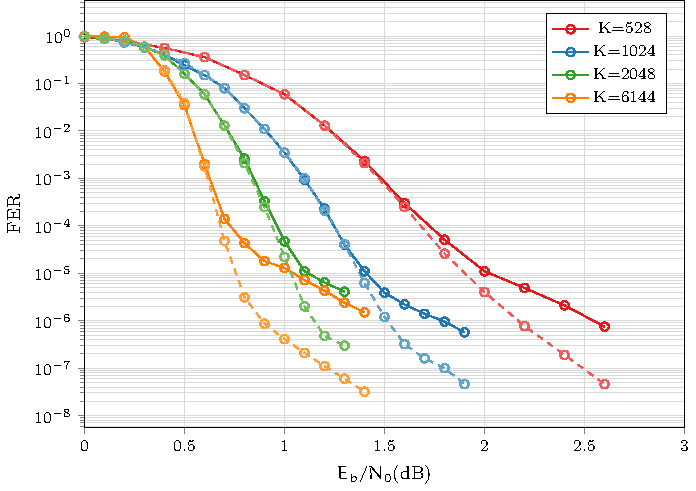
\includegraphics[width=\textwidth]{main/ch3_fig/fnc/lte/tikz/lte.pdf}
	\caption{Comparaison de performances de décodages entre EML-MAP et FNC. Standard LTE, K=528, 1024, 2048 et 6144.
	Décodeurs itérant jusqu'à 8 fois. \label{fig:fnc_lte}}
\end{figure}

Pour ces quatre cas considérés, l'amélioration du processus de turbo décodage obtenu par l'algorithme FNC représente un
gain en terme de FER au moins égal à un ordre de grandeur dans la zone du plancher d'erreur. Cela signifie qu'au moins 
$90\%$ des trames erronées sont corrigées par l'approche FNC. Le Tableau \ref{tab:fnccomp} compare le taux d'erreur trame 
attendu en extrapolant les performances de la métrique présenté en section précédente et celui réellement obtenu avec 
l'algorithme FNC l'utilisant pour $q=10$. Ces données se basent sur celles de la Figure \ref{fig:idLTE}. 
Cependant, comme le code CRC n'était pas utilisé dans le décodage, il n'était pas comptabilisé dans le rendement. En 
revanche dans les courbes de la Figure \ref{fig:fnc_lte} il l'est soit en tant que 
critère d'arrêt, soit dans le processus FNC. Un décalage de la valeur du SNR par 
$10\times \log_{10}\left(\frac{K}{K-24}\right)$
est alors ajouté aux données de la Figure \ref{fig:idLTE} pour pouvoir les exploiter.
\begin{table}[]
\centering
\caption{Comparaison entre les valeurs de taux d'erreur trames attendues avec une correction parfaite et celui réellement obtenu}
\label{tab:fnccomp}
\begin{tabular}{@{}lrrrr@{}}
\toprule
    & \begin{tabular}[c]{@{}l@{}}\textbf{K=528}  \\ @ 2.6 dB\end{tabular} & \begin{tabular}[c]{@{}l@{}}\textbf{K=1024} \\ @ 1.6 dB\end{tabular} & \begin{tabular}[c]{@{}l@{}}\textbf{K=2048} \\ @ 1.35 dB\end{tabular} & \begin{tabular}[c]{@{}l@{}}\textbf{K=6144} \\ @ 0.82 dB\end{tabular} \\ 
    \cmidrule(l){2-2}\cmidrule(l){3-3}\cmidrule(l){4-4}\cmidrule(l){5-5}
FER EML-MAP     & 7 e-7           & 2.3e-06         & 3e-6             & 4e-5             \\
BE < 10  		& 98\%            & 94\%            & 97\%             & 97\%             \\
FER attendu     & 1.4e-8          & 1.4e-7          & 9e-8             & 1.2e-6             \\
FER FNC         & 5e-8            &                 & 2e-7             & 2e-6             \\ \bottomrule
\end{tabular}
\end{table}
% D'après ce tableau, il est visible que l'écart entre le taux d'erreur trame attendu et celui obtenu 
% est relativement faible. 
%Ceci démontre le choix judicieux réalisé précédemment dans le choix des valeurs de $I_\text{min}$.
%En effet, de la sorte, le code CRC n'a pas d'impact négatif sur la zone du plancher d'erreur induit par les faux positifs.
À la vue des performances obtenues vis-à-vis de celles attendues, nous pouvons statuer sur l'absence de 
dégradations due à d'éventuels faux positifs émanant de la détection via le code CRC. Ceci provient conjointement de sa
distance minimale suffisamment importante (provenant directement de sa taille) et de l'adaptation de $I_{\text{min}}$ en 
fonction de la taille de la trame.

Concernant le taux d'erreur binaire, les gains sont légèrement moins importants que ceux présentés pour le taux d'erreur trame. En effet,
de part son principe, l'algorithme FNC corrige les trames à faible nombre d'erreurs binaires. Ainsi, les trames erronées 
après processus FNC possèdent un nombre important d'erreurs binaires. Néanmoins, des gains d'environ un ordre de grandeur 
sont observés dans tous les cas considérés. 

La Figure \ref{fig:fnc_ccsds} présente les performances de l'algorithme FNC cette fois dans le contexte d'un turbo code 
du standard CCSDS. Les conditions sont les suivantEs. La taille de la trame vaut 1784 et le rendement nominatif R=1/3 est 
considéré. Le turbo décodeur itère jusque 10 fois. Le code CRC définit dans le standard CCSDS possède une longueur de 16.
Ainsi son pouvoir de détection d'erreurs est plus faible que celui du standard LTE. Aussi, les turbo codes du 
standard CCSDS possèdent une longueur de contrainte de 5. Cela implique que le nombre moyen d'itérations pour décoder une trame dans 
la zone du plancher d'erreur est plus élevé que dans le contexte LTE. Suite à ces deux constatations, la valeur de 
$I_\text{min}$ se doit d'être plus élevée que précédemment. Elle est donc fixée à 5 afin de ne pas être limitée par le code CRC. 
Il est visible que dans ce contexte, les gains sont légèrement moins important que pour le standard LTE. Néanmoins, ces gains
sont proches de l'ordre de grandeur.

\begin{figure}[!b]
	\centering
	\includegraphics[width=\textwidth]{main/ch3_fig/fnc/ccsds/tikz/ccsds.pdf}
	\caption{Comparaison de performances de décodages entre EML-MAP et FNC. Standard CCSDS, K=1784.
	Décodeurs itérant jusqu'à 10 fois. \label{fig:fnc_ccsds}}
\end{figure}

Par cet exemple, nous entrevoyons une limite du principe FNC. En effet, si le code CRC définit par le standard considéré 
possède un risque considérable d'erreur non détectée, alors ce dernier est limitant dans les gains de décodage obtenu
avec l'algorithme FNC. Maintenant, un comparaison avec l'état de l'art de la réduction de la zone du plancher d'erreur 
par des approches basées sur un post-traitement est dressée.

\subsubsection{Comparaison avec l'état de l'art}
\paragraph*{Performances de décodage}
Dans le chapitre premier, diverses méthodes permettant d'abaisser le plancher d'erreur des turbo codes ont été présentées.
Il s'agit des méthodes FSM (ou CIM), de la concaténation en série d'un code BCH et enfin du décodage par liste. 
Les méthodes de décodages par listes et FSM sont dépendantes d'un code détecteur d'erreurs, comme le principe FNC. Ainsi, 
pour obtenir la comparaison la plus juste dans la Figure qui va suivre, la courbe de référence, considérera un turbo code 
sans concaténation de CRC, bien que celui-ci est déjà présent dans la majorité de standards utilisant un turbo code. 
Ceci permet de ne pas désavantager l'approche considérant une concaténation avec un code BCH pouvant aussi agir comme 
code détecteur d'erreur.

Dans \cite{cim}, les performances de décodage de la méthode CIM sont présentées en prenant pour cadre un turbo code ayant pour
polynôme générateur $(13,15)_8$. La taille de la trame vaut 1504. Le turbo décodeur implémente l'algorithme EML-MAP et
itère 16 fois. Cependant dans cette publication, la détection d'erreurs est réalisée par un génie. C'est-à-dire
que la décision du décodeur est comparée avec la trame émise. Afin de considérer un cas pratique, le génie doit être remplacé
par un code CRC. Dans la Figure \ref{fig:fnc_soa}, nous considérons pour ce cas le code CRC du standard LTE, de taille 24.
La courbe de performances est donc translatée vers la droite de $10\times\log_{10}\left(\frac{1504}{1504-24}\right)=0.7\text{ dB}$.
Pour des raisons de complexité calculatoire qui seront détaillées plus loin, seul le cas correspondant au maximum à un 
turbo décodage supplémentaire (CIM(1)) est considéré. Dans ce cas, les performances de cette méthode et celles de l'algorithme
FNC sont semblables.

Dans \cite{andersenBCH}, un code BCH est concaténé avec le turbo code dans le but de corriger les erreurs résiduelles 
après le processus de turbo décodage. Dans la Figure \ref{fig:fnc_soa}, cette technique est explorée. La capacité de 
correction d'un code BCH est directement donnée par la quantité d'information redondante (cf. Chapitre Premier). Or, cet 
ajout abaisse la rendement du code. En résulte alors un décalage de la courbe de performance dans la zone de convergence 
vers la droite. Deux codes BCH différents sont testés : l'un corrigeant toutes les trames contenant 4 erreurs ou moins (t=4), l'autre 
corrigeant celles contenant 10 erreurs ou moins (t=10). Dans le premier cas, les performances dans la zone du plancher 
d'erreur sont moins intéressantes que celles obtenues par l'algorithme FNC. Il faut en effet que le code BCH ait un pouvoir
de correction de 10 pour obtenir les mêmes performances que l'algorithme FNC dans la zone du plancher d'erreur. Cependant, 
dans ce cas, la pénalité de convergence vaut 0.33 dB. Son utilisation dans un contexte de communications numériques 
est alors compromis. L'emploi d'un tel code concaténé peut néanmoins avoir avec un intérêt pour des tailles de trames
conséquentes. En effet la taille de l'information redondante est lié au logarithme en base 2 de la taille de trame.
C'est la raison pour laquelle un tel schéma a été choisi avec le code LDPC du standard DVB-S2.

\begin{figure}[!htb]
	\centering
	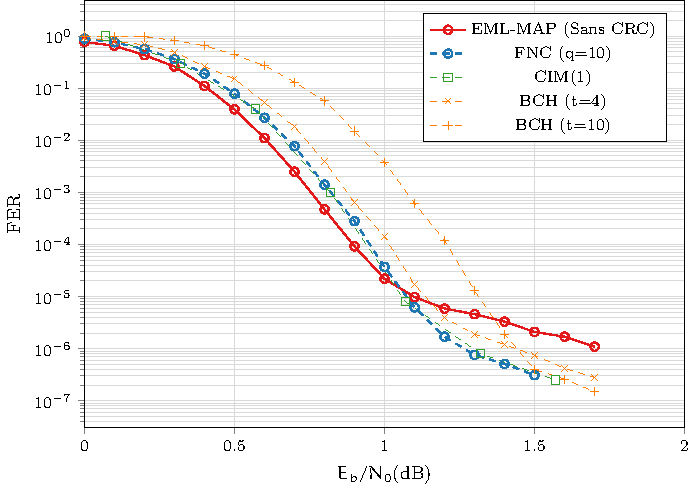
\includegraphics[width=\textwidth]{main/ch3_fig/fnc/soa/tikz/soa.pdf}
	\caption{Comparaison de performances de décodages entre EML-MAP, FNC, CIM et concaténation avec BCH. K=1784 et générateur
	polynomial $(13,15)_8$.	Décodeurs itérant jusqu'à 16 fois. \label{fig:fnc_soa}}
\end{figure}

\paragraph*{Complexité calculatoire} Selon \cite{david_gnaedig_thesis}, les calculs nécessaires pour qu'un turbo décodeur 
effectue une itération de l'algorithme EML-MAP pour un turbo code à 8 états s'établissent à $130\times K$ additions et 
et $62\times K$ opérations de comparaison et sélection.

Pour chaque itération, l'algorithme FNC est basé sur deux opérations principales. Tout d'abord, il s'agit de l'extraction 
des positions les moins fiables. Ceci peut être réalisé par un tri par insertion. Il nécessite alors $(K-q)\times q$ 
opérations de comparaison. Ensuite les $2^q$ vérifications du code CRC doivent avoir lieu. Pour implémenter chacun d'eux,
dans le cas du standard LTE, 24 bascules D sont nécessaires ainsi que 13 portes ou-exclusif. De la sorte, même si le 
nombre de calculs cd CRC croit exponentiellement avec $q$, il reste relativement faible en comparaison du nombre 
d'opérations nécessaires à chaque itération du turbo décodeur.

L'approche CIM(1) repose sur l'emploi de deux processus de turbo décodage successifs. Sa complexité calculatoire est donc
égale à deux fois celle d'un turbo décodage classique. A cela, il faut rajouter le tri nécessaire des valeurs, qui est 
le même que pour l'algorithme FNC. Aussi, il est à noter que l'approche FNC n'est pas à proprement parler un algorithme 
de post-traitement. En effet, son application sur les données produites par le turbo décodeur à l'itération $i$ peut être 
envisagé lors de l'itération $i+1$. De la sorte, il n'impacte que peu la latence du système, contrairement au CIM qui ne 
peut qu'effectuer le post-traitement après la fin du premier processus de décodage. Cette notion sera développé en détail
dans le prochain chapitre.

Enfin, en ce qui concerne la concaténation avec un code BCH, le décodage de ce dernier est basé sur l'emploi de l'algorithme
de Berlekamp-Massey suivi pas celui de Chien. Ces algorithmes reposent sur des additions et multiplications dans le corps
de Galois $GF(2^{\log_2 K})$, qui possèdent une complexité calculatoire relativement importante. Aussi, quelques additions
et opérations de comparaison et sélection sont nécessaires (respectivement $t\times K$ et $6T\times K$). Le tableau \ref{tab:cplx_soa}
reprend l'ensemble de ces données en présentant les applications numériques pour le contexte de la Figure \ref{fig:fnc_soa}.
C'est-à-dire pour un turbo code 8 états avec K=1504 et R=1/3 et un processus de décodage itérant 16 fois. 

\begin{table}[!t]
    \centering
    \caption{Comporaison de la complexité calculatoire pour $K=1504$, $I_{TC}=16$, $I_{min}=3$ et $t=10$ }
    \label{tab:cplx_soa}
    %\resizebox{\linewidth}{!}{
        \begin{tabular}{rllll}
            \toprule
            		& TDec 			& TDec + FNC 	& TDec + CIM(1) & TDec + BCH \\
            \cmidrule(l){2-2}\cmidrule(l){3-3}\cmidrule(l){4-4}\cmidrule(l){5-5}
            Add 	& $3~128~320$ 	& $$ 	& $6~256~640$ 	& $3~143~380$ \\
            CS  	& $1~491~968$ 	& $1~697~488$ 	& $$ 	& $1~492~028$ \\
            CRC 	& $13$      	& $13~312$   	& $26$      	& $0$       \\
            Add GF$\left(2^{11}\right)$ & $0$ & $0$ &$0$& $13~000$ \\
            Mul GF$\left(2^{11}\right)$ & $0$ & $0$ &$0$& $30~243$ \\
            \bottomrule
        \end{tabular}%}
\end{table}

\subsubsection{Conclusions}
L'algorithme Flip'N'Check pour les turbo codes binaires a été présenté. Celui-ci permet d'abaisser le plancher d'erreur 
des turbo codes binaires d'au moins une décade. Ses performances sont peu éloignées de celles obtenables via une 
identification parfaite. La complexité calculatoire de cet algorithme réside dans les vérifications du code CRC, dont leur 
nombre croit exponentiellement avec la profondeur de recherche des positions les moins fiables. Toutefois, une 
comparaison avec l'état de l'art a établit que son surcoût calculatoire est raisonnable tout en fournissant de très bonnes 
performances de décodage. Finalement, cette méthode peut s'adapter à des turbo codes standardisés dès lors qu'un code 
correcteur d'erreur y est concaténé en série. Maintenant, une adaptation aux turbo codes double binaires est détaillée.


\subsection{Applications aux turbo codes double binaire}
Cette section propose une transposition de l'algorithme FNC au cas double binaire. Après avoir décrit les transformations 
nécessaires, l'algorithme adapté au turbo codes double binaire est exprimé. Enfin, une présentation des performances obtenues 
est réalisée.
\subsubsection{Les adaptations}
Lors de la comparaison des métriques d'identification effectuée au début de ce chapitre, plusieurs propositions ont été 
comparée. L'une d'entre elle, la métrique $\Delta'_1$, possède les meilleurs performances d'identification. C'est donc
elle qui est retenue pour cette adaptation. Cependant, dans le cas double binaire, les positions identifiées correspondent 
à des symboles. Chacun d'entre eux représente alors 4 symboles différents. Suivant cette constatation, une adaptation directe 
requerrait alors la génération de $4^q$ mots candidats. Le nombre de vérifications du code CRC ayant la même valeur, 
uniquement de faibles valeurs de $q$ pourrait être considérées. Or, d'après les statistiques d'identification présentées en Figure 
\ref{fig:dvb752}, afin de pouvoir observer une amélioration notable des performances de décodage, le choix de $q$ semble
devoir se porter \textit{a minima} à 8. Dans ce cas, 65536 vérifications de CRC seraient alors à réaliser, ce qui est 
irréaliste pour un contexte de communications numériques contraint.

Il est alors nécessaire de réduire le nombre de symboles testés par position identifiée. Pour ce faire une analyse à été 
menée quant à l'identification du bon symbole grâce à un génie. Cette identification est semblable à celle permettant 
l'extraction des positions les moins fiables.
Soient $S_{M_x}(k)$, $S_{M_y}(k)$, $S_{M_z}(k)$, et $S_{M_t}(k)$ respectivement le symbole le plus probable au sens 
des informations \textit{a posteriori}, le second symbole le plus probable, le troisième et enfin le symbole le moins 
probable. Ils ont alors pour expression :
\begin{align*}
S_{M_x}(k) &= \argmax\limits_{s\in\llbracket0;3\rrbracket}\left(l^a_s(k)\right) \\
S_{M_y}(k) &= \argmax\limits_{s\in\llbracket0;3\rrbracket\setminus{S_{M_x}(k)}}\left(l^a_s(k)\right)\\
S_{M_z}(k) &= \argmax\limits_{s\in\llbracket0;3\rrbracket\setminus{\{S_{M_x}(k)}, S_{M_y}(k)\}}\left(l^a_s(k)\right)\\
S_{M_t}(k) &= \{0,1,2,3\}\setminus{\{S_{M_x}(k), S_{M_y}(k), S_{M_z}(k)\}}
\end{align*}
Le tableau \ref{tab:symb} présente des statistiques quant à l'index du symbole réellement transmis lorsque le symbole 
considéré est erroné à l'issu de l'itération courante. Ces statistiques ont été été obtenues avec différents turbo
codes du standard DVB-RCS. Ce tableau présente le nombre de fois où pour chaque trame erronée l'ensemble des erreurs 
correspond au symbole $S_{M_x}$, ou correspond au symbole $S_{M_y}$ ou au symbole $S_{M_x}$, en continuant de la sorte en 
réunissant les ensembles. Cela permet d'observer quels doivent être les symboles considérés lors de la génération des 
mots candidats. Nous pouvons constater que la première colonne vaut toujours 0\% puisque le symbole le plus probable correspond au
symbole décodé. Cependant, il est à noter que si l'information \textit{a posteriori} doit être reconstruite (cas où le 
décodeur SISO fournit en sortie l'information extrinsèque et le vecteur décidé) le facteur de remise à l'échelle doit 
être bien pris en compte pour calculer l'index des symboles. En effet, l'identification via la métrique $\Delta'$ réussi 
en raison du faible l'écart entre les valeurs \textit{a posteriori}. Ainsi, une légère modification dans leurs calculs 
modifie grandement la trame décodée. Il serait alors possible de constater que le symbole le plus probable calculé ne
soit pas celui décodé.
\begin{table}[!tb]
    \centering
    \caption{Statistiques sur le symbole transmis vis-à-vis des différents symboles possibles}
    \label{tab:symb}
    %\resizebox{\linewidth}{!}{
        \begin{tabular}{rllll}
            \toprule
            		& $S_{M_x}$	& $S_{M_x}\cup S_{M_y}$	& $S_{M_x}\cup S_{M_y}\cup S_{M_z}$ & $S_{M_x}\cup S_{M_y}\cup S_{M_z}\cup S_{M_t}$ \\
            \cmidrule(l){2-2}\cmidrule(l){3-3}\cmidrule(l){4-4}\cmidrule(l){5-5}
            i=3     &	0\%		&	96\%	& 	3\%		&	1\%		\\
            i=4     &	0\%		&	96\%	& 	3\%		&	1\%		\\
            i=5     &	0\%		&	97\%	& 	3\%		&	0\%		\\
            i=6     &	0\%		&	97\%	& 	3\%		&	0\%		\\
            i=7     &	0\%		&	97\%	& 	3\%		&	0\%		\\
            i=8     &	0\%		&	97\%	& 	2\%		&	1\%	\\
            \bottomrule
        \end{tabular}%}
\end{table}
 
Par les données présentées dans ce tableau, il apparaît que dans la très grande majorité des cas, le symbole transmis 
correspond au symbole le deuxième plus probable. Considérer les deux symboles les moins probables ne permet alors 
d'augmenter la probabilité de fournir le bon mot de code que d'une part marginale alors que la complexité calculatoire
induite serait sévère.

Finalement, de part cette analyse, considérer uniquement les deux symboles les plus probables est suffisant pour 
pouvoir identifier le bon mot de code. Le nombre de vérifications de code CRC reste alors constant avec le cas binaire 
et vaut $2^q$. Une étape supplémentaire consistant à l'extraction des deux symboles les plus probables est néanmoins 
nécessaire. Il est maintenant possible de proposer l'algorithme complet, sujet de la prochaine sous-section.

\subsubsection{Détail de l'algorithme}
L'algorithme FNC pour les turbo codes double binaires est fortement semblable à celui du cas binaire. Seules quelques 
opérations supplémentaires apparaissent. Un détail en est maintenant donné. Tout d'abord, $I_{\text{min}}$ itérations de 
turbo décodages seules sont effectuées. Ceci permet de réduire le risque d'erreurs non détectées lors de la vérification 
du code CRC. À partir de l'itération suivante, le code CRC commence à être vérifié. S'il ne l'est pas, le principe FNC
est alors appliqué. D'abord, pour chaque position symbole dans la trame, les deux symboles les plus probables sont 
extraits au sens de l'information \textit{a posteriori}. Ceci permet de calculer la métrique $\Delta'$. Une fois que 
tous ses indices ont été calculés, les $q$ positions des symboles les moins fiables sont extraits en triant par ordre 
croissant la métrique $\Delta'$. Ces positions sont stockées dans $\Omega$. Ensuite, à partir des positions contenus dans
$\Omega$ et des indices de $S_{M_x}$ et $S_{M_y}$, la valeur des deux symboles les plus probables sont extraits pour 
chacune des positions présupposée erronée. Reste à générer les $2^q$ mots candidats en remplaçant la valeur des symboles
aux positions correspondantes dans le mot produit par le turbo décodeur. Finalement, ces mots candidats sont vérifiées
en utilisant le code CRC. Si un mot le vérifiant est trouvé, alors le processus est stoppé. Sinon une nouvelle itération
du processus de turbo décodage est effectuée. L'algorithme \ref{alg:fc_db} récapitule l'ensemble de ces opérations.

L'algorithme FNC dans le contexte de turbo codes double binaires nécessite donc plus d'opérations que dans le cas binaire.
Ceci provient directement de la manipulation de symboles. Ainsi, l'opération d'extraction nécessaire des deux symboles 
les plus probables correspond à un manipulation pour l'hypothétique correction de deux bits. Ainsi, la complexité globale
de l'algorithme par bit décodé n'est que peu modifiée.\\
Afin de réaliser ces deux extractions de valeurs maximum (correspondant aux lignes 9, 10 et 13 de l'algorithme 
\ref{alg:fc_db}), un réseau de trie peu être utilisé. Dans ce cas, pour chaque symbole, 5 comparaisons sont nécessaires.
En utilisant la décision du turbo décodeur, il est possible de réduire le nombre de comparaison à 3. Mais dans ce cas,
de la logique supplémentaire sera nécessaire afin de sélectionner les entrées de ces 3 comparateurs. Comme ces opérations
ne sont réalisé qu'une fois par itération, leur impact sur la complexité globale est faible. Maintenant, une présentation
des performances de décodage dans le contexte des standards DVB-RCS et DVB-RCS2 est réalisée.
\begin{center}
\begin{minipage}{.95\textwidth}%
\begin{algorithm}[H]
\label{alg:fc_db}
	\DontPrintSemicolon
	\SetKwFunction{TD}{Itération de Turbo Décodage}
	\SetKwFunction{GC}{Génération du mot candidat}
	\SetKwFunction{L}{Extraction des positions des symboles moins fiables}
	\SetKwFunction{S}{Extraction des 2 symboles les plus fiables}
	\SetKwFunction{R}{return}
	\SetKwFunction{CRC}{CRCheck}
	
	\For{i: 1 à  $I_{min}$}{
		\TD\;
	}
	\For{i: $I_{min}+1$ to  $I_{TC}$}{
		$\left(\mathbf{\hat{{d}}}, \mathbf{L}\right)$ = \TD\;
		\If{\CRC{$\mathbf{\hat{{d}}}$}==true}{
			\R{$\hat{{d}}$}\;
		}
		\Else{
			\For{k: 1 à K}{	
				$S_{M_x}(k) = \argmax\limits_{s\in\llbracket0;3\rrbracket}\left(l^a_s(k)\right)$\;
				$S_{M_y}(k) = \argmax\limits_{s\in\llbracket0;3\rrbracket\setminus{S_{M_x}(k)}}\left(l^a_s(k)\right)$\;
				$\Delta'_k = l^a_{S_{M_x}}(k)-l^a_{S_{M_y}}(k)$\;		%
			}
			$\Omega =$ \L{$\Delta$, q}\;
			$\xi =$ \S{$\Omega$, $S_{M_x}$, $S_{M_y}$}\;
			\For{j: 1 à $2^q-1$}{								
				$\mathbf{D} =$\GC{$\Omega, \xi, j, \mathbf{\hat{d}}$}\;
				\If{\CRC{$\mathbf{D}$}==true}{
					\R{$\mathbf{D}$}\;
				}
			}
		} %end else
	}
	\R{$\hat{{d}}$}\;
	\caption{L'algorithme Flip and Check pour les turbo codes double binaires}
\end{algorithm}
\end{minipage}
\end{center}


\subsubsection{Performances de décodage}
Dans cette section le résultat de simulations Monte Carlo réalisés avec une représentation des données en virgule
flottante sont détaillés. Un canal AWGN est toujours considéré. En revanche, la modulation est maintenant une QPSK. Le 
nombre d'itérations maximum réalisées par le turbo décodeur est fixé à 8 et $I_{\text{min}}$ vaut 3.
Comme dans le cas binaire, la valeur de $q$ est fixée à 10. Dans le standard DVB-RCS, les tailles de trame s'étalent 
de quelques dizaines d'octets à 200 octets. Sept rendements différents sont définis allant de 1/3 à 6/7. Le code CRC 
considéré dans ce standard est de longueur 16. La Figure \ref{fig:fnc_dvb1_440} compare les performances du turbo décodage
conventionnel et du celles de l'algorithme FNC pour K=440 symboles et pour différentes valeurs de rendement. Il apparaît 
ainsi que grâce à l'algorithme FNC, dans la zone du plancher d'erreur, le turbo code de rendement 1/2 possède de 
meilleures performances que celles obtenues pour le turbo code de rendement 1/3 avec un décodage conventionnel EML-MAP. 
Plus généralement, pour des valeurs de SNR moyennes à élevées, quelque soit le rendement du code, l'algorithme FNC apporte 
des gains au moins égaux à un ordre de grandeur. En terme de SNR, cela correspond à des gains allant de 0.4 dB à plus de 
0.6 dB.

Pour les autres tailles de trames de standard, les gains sont tout aussi conséquents et équivalents. Pour confirmer ces
dires, des courbes de performances présentant le taux d'erreur trame obtenu avec l'algorithme FNC sont présentés en 
Annexe \ref{ann:fnc}. Il apparaît que la pente de la courbe dans la zone du plancher d'erreur est modifiée, l'inflexion
est moins importante grâce à l'algorithme FNC.

\begin{figure}[!htb]
	\centering
	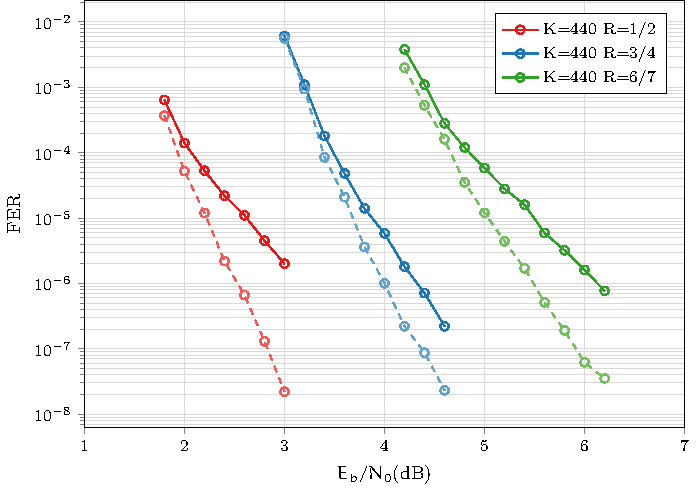
\includegraphics[width=\textwidth]{main/ch3_fig/fnc/dvb/tikz/dvb1_440.pdf}
	\caption{Comparaison de performances de décodages entre EML-MAP et FNC. Standard DVB-RCS, K=440, Rendement de 1/3 à 
	6/7. Décodeurs itérant jusqu'à 8 fois. \label{fig:fnc_dvb1_440}}
\end{figure}
En 2012, le successeur du standard DVB-RCS a été publié. Le code correcteur considéré est toujours un turbo code double
binaire. En revanche, afin d'améliorer les performances de corrections, la longueur de contrainte des codes constituants
est augmentée. Des turbo codes 16 états sont alors considérés. Un nouvel entrelaceur ARP ainsi que des tailles de trame
plus conséquentes sont définis. La taille du code CRC concaténé en série double, pour passer à une profondeur de 32. 
Enfin de nouveaux schémas de poinçonnage sont ajoutés. De la sorte, ces turbo codes font 
partis des codes correcteurs les plus performants et flexibles standardisés. La complexité calculatoire de ce code a
toutefois doublé en comparaison de celle du turbo code de la génération précédente. 

\begin{figure}[!htb]
	\centering
	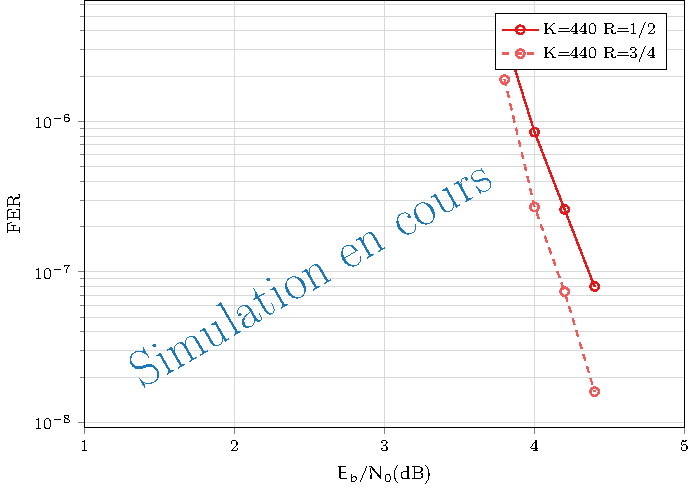
\includegraphics[width=\textwidth]{main/ch3_fig/fnc/dvb2/tikz/dvb2.pdf}
	\caption{Comparaison de performances de décodages entre EML-MAP et FNC. Standard DVB-RCS 2, K=752, Rendement de 1/2 à 
	4/5. Décodeurs itérant jusqu'à 8 fois. \label{fig:fnc_dvb2_752}}
\end{figure}

La Figure \ref{fig:fnc_dvb2_752} présente une comparaison des performances de décodage pour le standard DVB-RCS 2 avec
K=752. Différents rendements sont considérés : 1/2, 2/3, 3/4 et 4/5. Les autres paramètres de la simulation restent les
même que pour le cas 8 états.
Tout d'abord, en considérant un décodage conventionnel, il apparaît que les performances de ce code surpassent très largement 
celles du DVB-RCS. En effet, les points d'inflexions des différentes courbes de performances apparaissent 2 à 3 décades
plus bas. La zone du plancher d'erreur correspond alors à des taux d'erreur trame de l'ordre de $10^{-7}$. Ceci entraîne
un temps nécessaire pour les simulations Monte-Carlo conséquent. D'autant plus, le FNC visant à abaisser le plancher 
d'erreur, apercevoir une trame erronée devient alors extrêmement rare. Ainsi les courbes obtenues n'ont compté que 30 
trames erronées avec l'algorithme FNC.

Il apparaît que même dans un contexte de turbo code très performants, des gains conséquents dans la zone du plancher d'erreur 
sont obtenus grâce à l'emploi de l'algorithme FNC. À nouveau, un changement de la pente de la courbe dans cette zone est
visible. Ceci à pour conséquence de fournir des gains approchant la décade dans certains cas comme pour R=4/5. Dans d'autres
cas, comme pour R=1/2, les gains dépassent légèrement l'ordre de magnitude.
% PERFS++

\section{Conclusions}
Dans ce troisième chapitre, une étude sur les erreurs résiduelles des turbo codes a été menée. Dans un premier temps,
leur existence a été caractérisée grâce aux spectres de distances des turbo codes. Ces erreurs étant responsables de 
la zone du plancher d'erreur, des propositions de critères d'identifications ont alors été comparés.

Cette comparaison a permis de mettre en exergue une métrique, permettant d'identifier de façon quasi systématique
les erreurs résiduelles à l'issue du processus de turbo décodage. À partir de celle-ci, un algorithme, nommé Flip'N'Check
a été proposé. Cet algorithme tire parti de l'augmentation de la distance minimale obtenue via la concaténation en série 
d'un code détecteur d'erreur et d'un turbo code. Un tel schéma de codage est couramment rencontré dans les standards de 
communications. Le principe de cet algorithme repose sur l'identification des positions les moins fiables dans la séquence en train 
d'être décodée. De là, différents mots de codes candidats sont générés puis vérifiés en utilisant le code détecteur d'erreurs.
Des gains d'au moins une décade ont été observés, ce, quelque soit le turbo code standardisé considéré. Ainsi, des gains
de performances conséquents sont observables pour des turbo codes binaires à 8 ou 16 états ainsi que pour des turbo codes 
double binaires eux aussi à 8 ou 16 états. La complexité calculatoire additionnelle nécessaire à cet algorithme est modérée.
Cela le rend alors intéressant face à l’état de l'art de la réduction du plancher d'erreurs des turbo codes.

Dans le chapitre suivant, après une étude des architectures matérielles de turbo décodeurs, des propositions d'implémentation 
de l'algorithme Flip'N'Check sont étudiées.


% Conclusion: Méthode relativement simple à mettre en oeuvre qui tire parti de l'auigmentation de la dmin du code grace a 
% la concat.
%PAS DE SPECTRE EN DOUBLE BINAIRE...
%CONFIRMER VALEURS TABLEAU FNC
%Gains obtenables par la méthode dépendent de la distribution de spectre d'erreur

%Parler métriques aposteriori binaires pour le double binaire => non présentées car moins performantes